\documentclass[../tc_tpfinal_main.tex]{subfiles}

\begin{document}

%capítulo
\chapter{Filtro}

\section{Introducción}

\section{Análisis de sensibilidades}
\subsection{Celda Sallen-Key Pasabandas}

			 	\begin{table}[H] 
				\centering
 				\begin{tabular}{||c c c c c c c c c||} 
 					\hline
				  Parámetro& $R_1$ & $R_2$ & $R_3$ & $R_4$ & $r_a$ & $r_b$&$C_1$&$C_2$\\ [0.5ex] 
 					\hline\hline
					 $S^G_x$& 1 & 0& -1& 0&0&0&0&0\\
					 $S^{w_0}_x$& $- \frac{1}{2}$ &$- \frac{1}{2}$& 0& 0&$- \frac{1}{2}$&$- \frac{1}{2}$&$- \frac{1}{2}$&$- \frac{1}{2}$\\
					 $S^{Q}_x$&$- \frac{1}{2}$ &$- \frac{1}{2}$& 0& 1&$- \frac{1}{2}$&$- \frac{1}{2}$&$- \frac{1}{2}$&$- \frac{1}{2}$\\[1ex] 
					\hline
				\end{tabular}
			\end{table}
\subsection{Celda Sallen-Key Pasa-altos}
\begin{figure}[H]	
	\centering
	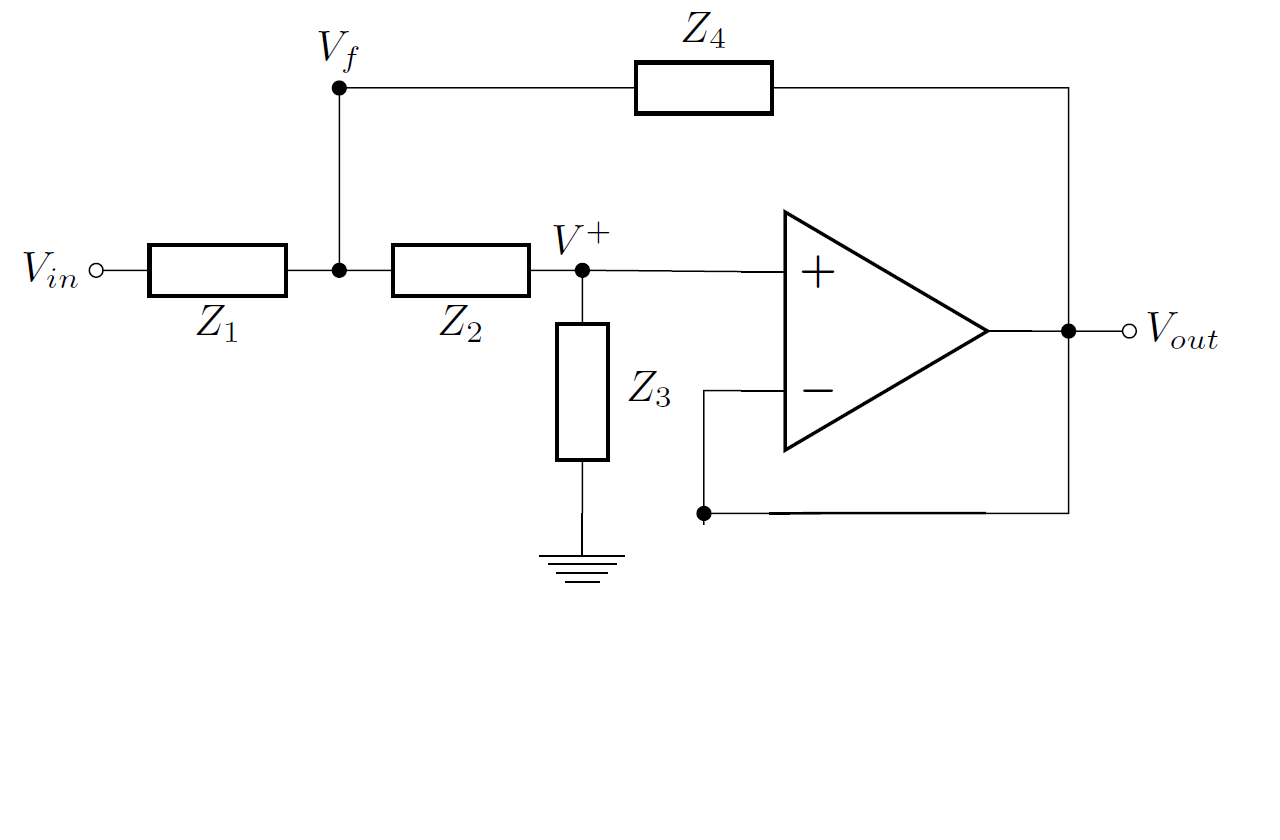
\includegraphics[scale=0.5]{imagenes/sallen_key_circ.png}
	\caption{Celda Sallen-Key Pasa-altos}
	\label{fig:tpfinal_sallen_key_circ}
\end{figure}
 	\begin{table}[H] 
				\centering
 				\begin{tabular}{||c c c c c c c c c||} 
 					\hline
				  Parámetro& $R_1$ & $R_2$ & $R_3$ & $R_4$ & $r_a$ & $r_b$&$C_1$&$C_2$\\ [0.5ex] 
 					\hline\hline
					 $S^G_x$& 1 & 0& -1& 0&0&0&0&0\\
					 $S^{w_0}_x$& $- \frac{1}{2}$ &$- \frac{1}{2}$& 0& 0&$- \frac{1}{2}$&$- \frac{1}{2}$&$- \frac{1}{2}$&$- \frac{1}{2}$\\
					 $S^{Q}_x$&$- \frac{1}{2}$ &$- \frac{1}{2}$& 0& 1&$- \frac{1}{2}$&$- \frac{1}{2}$&$- \frac{1}{2}$&$- \frac{1}{2}$\\[1ex] 
					\hline
				\end{tabular}
			\end{table}
\subsection{Celda Sallen-Key Pasa-altos con factor ganancia}
\begin{figure}[H]	
	\centering
	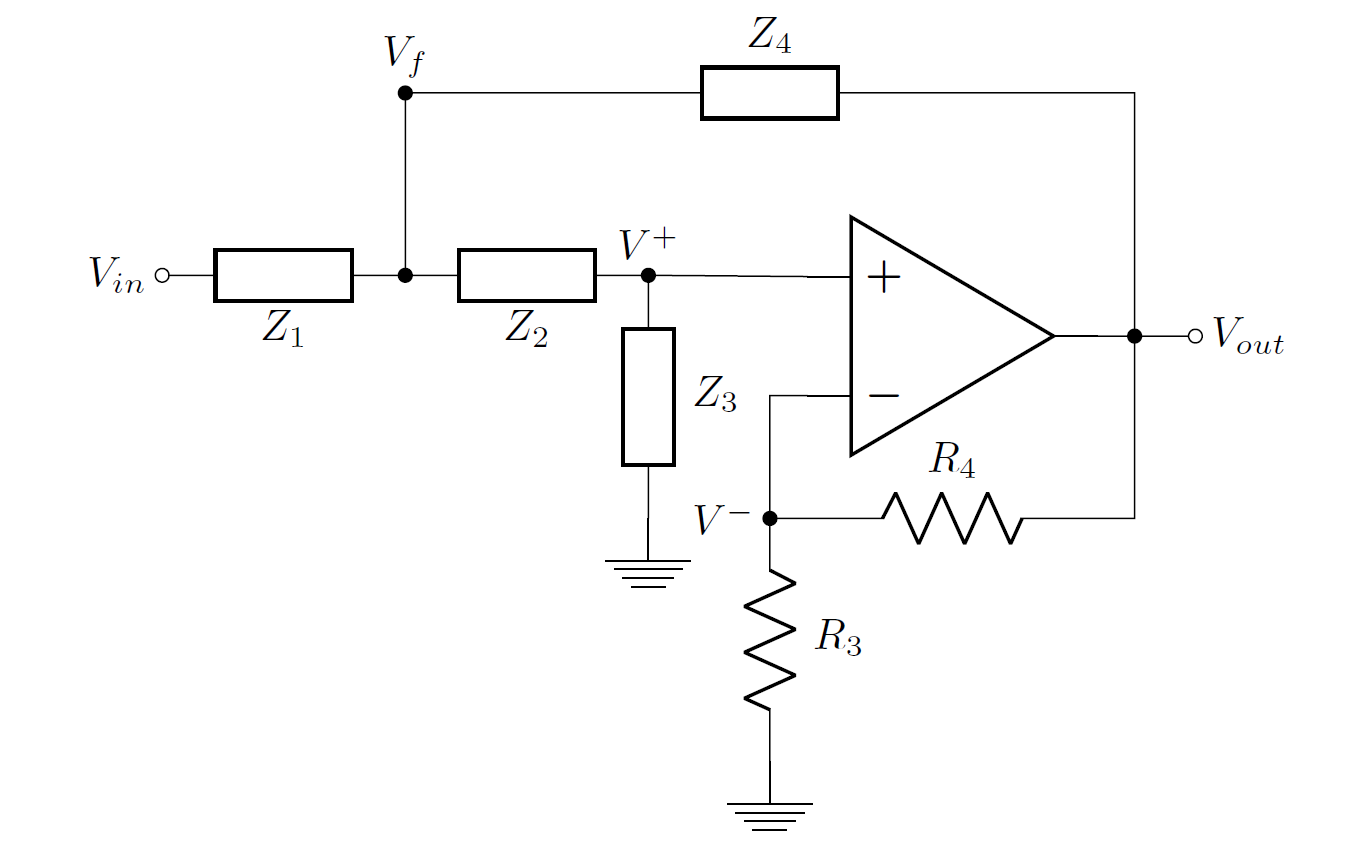
\includegraphics[scale=0.5]{imagenes/sallen_key_gain_circ.png}
	\caption{Celda Sallen-Key Pasa-altos con factor ganancia}
	\label{fig:tpfinal_sallen_key_gain_circ}
\end{figure}
			 	\begin{table}[H] %datos thd simulado
				\centering
 				\begin{tabular}{||c c c c c c c c c||} 
 					\hline
				  Parámetro& $R_1$ & $R_2$ & $R_3$ & $R_4$ & $r_a$ & $r_b$&$C_1$&$C_2$\\ [0.5ex] 
 					\hline\hline
					 $S^G_x$& 1 & 0& -1& 0&0&0&0&0\\
					 $S^{w_0}_x$& $- \frac{1}{2}$ &$- \frac{1}{2}$& 0& 0&$- \frac{1}{2}$&$- \frac{1}{2}$&$- \frac{1}{2}$&$- \frac{1}{2}$\\
					 $S^{Q}_x$&$- \frac{1}{2}$ &$- \frac{1}{2}$& 0& 1&$- \frac{1}{2}$&$- \frac{1}{2}$&$- \frac{1}{2}$&$- \frac{1}{2}$\\[1ex] 
					\hline
				\end{tabular}
			\end{table}
\subsection{Celda Tow-Thomas}

\begin{figure}[H]	
	\centering
	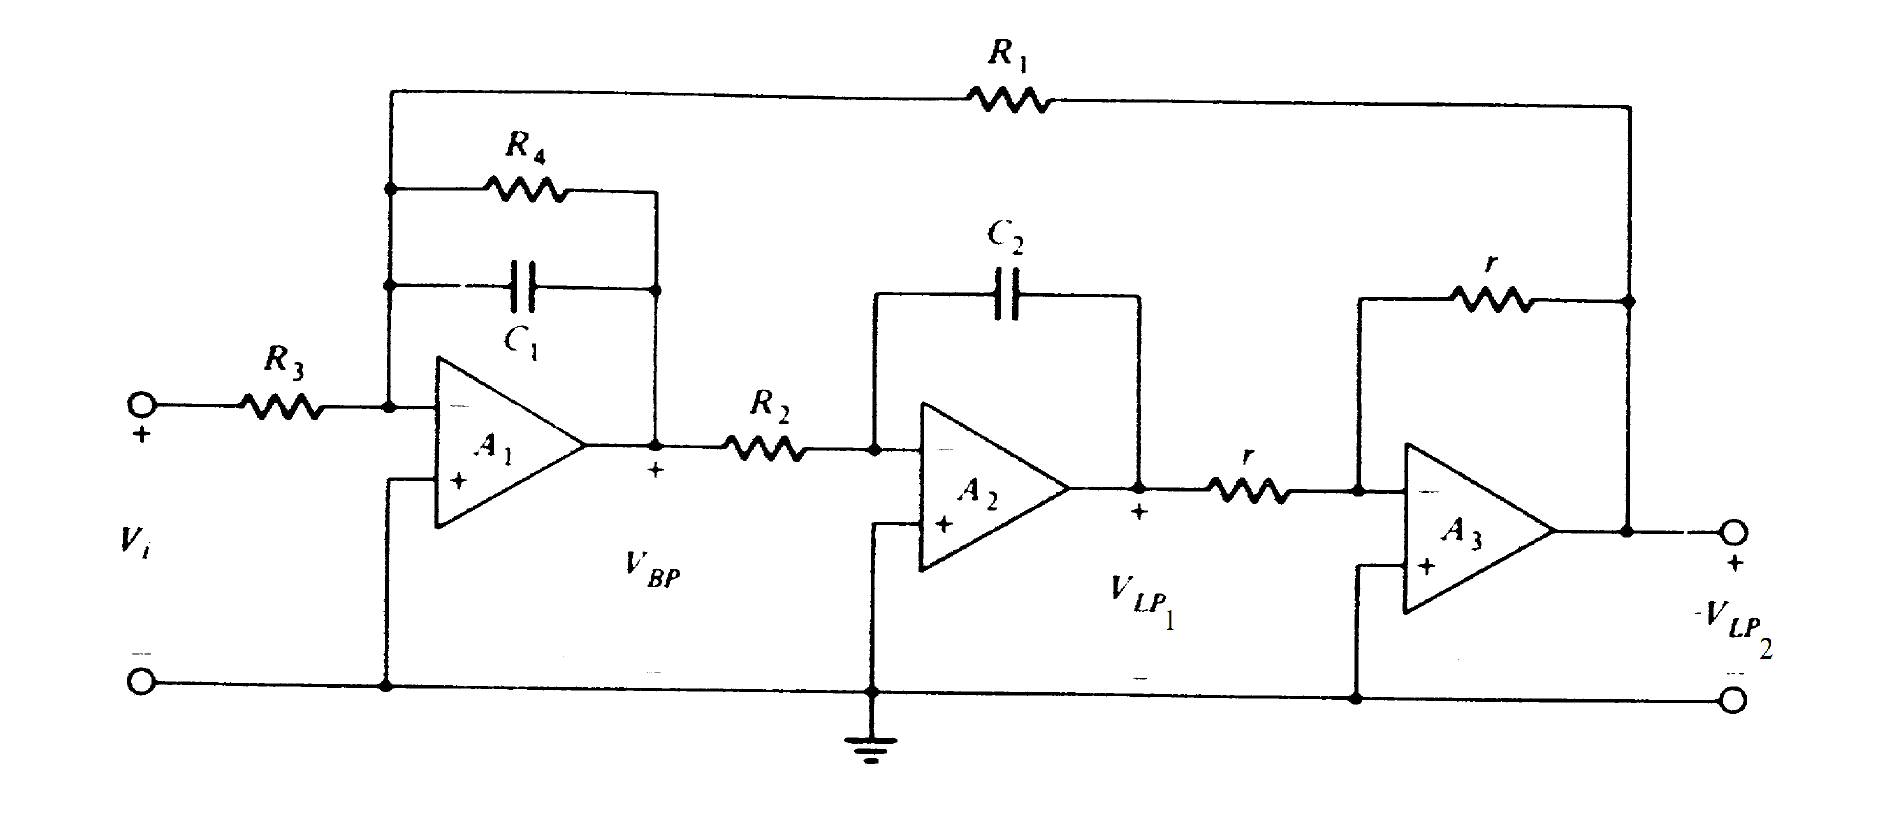
\includegraphics[scale=0.5]{imagenes/tow_thomas_circ.png}
	\caption{Celda Tow-Thomas}
	\label{fig:tpfinal_tow_thomas_circ}
\end{figure}

Se despeja la transferencia total del sistema:\par
\begin{center}
$H(s) = -\frac{\mathrm{R_1}\, \mathrm{R_4}\, \mathrm{r_b}}{\mathrm{R_3}\, \left(\mathrm{C_1}\, \mathrm{C_2}\, \mathrm{R_1}\, \mathrm{R_2}\, \mathrm{R_4}\, \mathrm{r_b}\, s^2 + \mathrm{C_2}\, \mathrm{R_1}\, \mathrm{R_2}\, \mathrm{r_a}\, s + \mathrm{R_4}\, \mathrm{r_b}\right)}
$
\end{center}

De la cual se despejan los siguientes parámetros:\par

\begin{center}
$w_0 = \sqrt{\frac{r_b}{C_1\cdot C_2\cdot R_1\cdot R_2\cdot ra}}; $
%wo = sqrt(rb/(c1*c2*r1*r2*ra))
$Q = \sqrt{\frac{C_1\cdot r_b}{C_2\cdot R_1\cdot R_2\cdot ra}}; $
%Q = r4*sqrt(c1*rb/(c2*r1*r2*ra));
$G = -\frac{R_1}{R_4}; $ 
\end{center}

Para la ganancia, obtenemos las sensibilidades con respecto a todos los componentes:\par

 	\begin{table}[H] %datos thd simulado
				\centering
 				\begin{tabular}{||c c c c c c c c c||} 
 					\hline
				  Parámetro& $R_1$ & $R_2$ & $R_3$ & $R_4$ & $r_a$ & $r_b$&$C_1$&$C_2$\\ [0.5ex] 
 					\hline\hline
					 $S^G_x$& 1 & 0& -1& 0&0&0&0&0\\
					 $S^{w_0}_x$& $- \frac{1}{2}$ &$- \frac{1}{2}$& 0& 0&$- \frac{1}{2}$&$- \frac{1}{2}$&$- \frac{1}{2}$&$- \frac{1}{2}$\\
					 $S^{Q}_x$&$- \frac{1}{2}$ &$- \frac{1}{2}$& 0& 1&$- \frac{1}{2}$&$- \frac{1}{2}$&$- \frac{1}{2}$&$- \frac{1}{2}$\\[1ex] 
					\hline
				\end{tabular}
			\end{table}
			


\end{document}